% Grossmont College -- Chem 141 Lab 6: Calorimetry
% Cameron Carroll
% March 2014


\documentclass[fleqn,titlepage]{article}

\renewcommand*\rmdefault{ppl}

\usepackage[version=3]{mhchem} % Package for chemical equation typesetting
\usepackage{tabu}
\usepackage{wasysym}
\usepackage{listings}
\usepackage{scrextend}
\lstset{language=Matlab}
\usepackage{multirow}

% set 1" margins on 8.5" x 11" paper
% top left is measured from 1", 1"
\topmargin 0in
\oddsidemargin 0in
\evensidemargin 0in
\headheight 0in
\headsep 0in
\topskip 0in
\textheight 9in
\textwidth 6.5in

\usepackage{graphicx} % Required for the inclusion of images

\setlength\parindent{0pt} % Removes all indentation from paragraphs

\renewcommand{\labelenumi}{\alph{enumi}.} % Make numbering in the enumerate environment by letter rather than number (e.g. section 6)

%\usepackage{times} % Uncomment to use the Times New Roman font

%----------------------------------------------------------------------------------------
% DOCUMENT INFORMATION
%----------------------------------------------------------------------------------------

\begin{document}

\begin{titlepage}
  \mbox{}\\[1.25cm]
  \textbf{\LARGE Cameron Carroll \\ Grossmont College}\\[2.25cm]
  \begin{center}
    \textbf{\huge Lab 6: \\ Calorimetry: Measuring Heat of Formation}\\[2.50cm]
  \end{center}
  \textbf{\LARGE Professor: Martin Larter \\ Chemistry 141-0692} \\
  \vfill
  \center{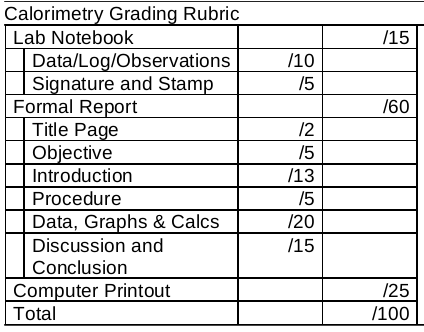
\includegraphics{./lab6_rubric}}
  \center{\textbf{\LARGE Performed --} {\LARGE March 13 \& 18, 2014}}
  \center{\textbf{\LARGE Submitted --} {\LARGE April 3, 2014}}
\end{titlepage}

%----------------------------------------------------------------------------------------
% SECTION 1
%----------------------------------------------------------------------------------------
\section*{Objective}
  \paragraph{} This experiment explores the use of calorimetry to measure heat capacity of the calorimeter apparatus itself and then to determine the heat of formation of a substance. Because directly measuring heat of formation of magnesium oxide would be difficult, we us an indirect measurement and Hess's law to get the result.

%----------------------------------------------------------------------------------------
% SECTION 2
%----------------------------------------------------------------------------------------
\section*{Introduction}
  \paragraph{} Calorimetry is a technique used to determine the heat of a reaction by capturing the change in heat of the surroundings, an indirect method more vible than direct measurement. The calorimeter, an apparatus which can be as simple as two nested coffee cups, has a known `calorimeter constant.' It absorbs a known amount of heat or a given temperature change, leaving the rest to be associated with the reaction. A few definitions:
  \begin{itemize}
    \item The  calorimeter constant is the heat capacity determined by mixing known amounts and temperatures of water and measuring the resulting change.
    \item The heat of formation is the heat associated with the formation of a substance from its constituent elements. In the case of \ce{MgO}, \ce{Mg + 1/2O_2 -> MgO}
  \end{itemize}

%----------------------------------------------------------------------------------------
% SECTION 3
%----------------------------------------------------------------------------------------
\section*{Procedure}
\begin{itemize}
  \item  \textbf{Referenced From:} \\
    \begin{addmargin}[1em]{1em}
      Lehman, J. (Et al), `Calorimetry: Measuring the Heat of Formation' \\
      Grossmont College, Chemistry 141 Lab Manual, 6th edition, pp 71-76 \\
      El Cajon, California
    \end{addmargin}
\end{itemize}

%----------------------------------------------------------------------------------------
% SECTION 3
%----------------------------------------------------------------------------------------
\section*{Data Summary \& Calculations}
  \paragraph{} (See next, handwritten, pages.)

%----------------------------------------------------------------------------------------
% SECTION 4
%----------------------------------------------------------------------------------------
\newpage
\section*{Discussion \& Conclusions}
\paragraph{} My data for the calorimeter constant was not close to the default; I'm not entirely sure what went wrong, even, but my value was 11\% off, so I used the default for my other calculations.
\paragraph{} I obtained a value of 601.8 KJ/mol, almost exactly the literature value. I expected to be off significantly due to a couple experimental errors: First of all, some of the \ce{Mg} and \ce{MgO} stuck to the sides of the calorimeter cup and werent incorporated into the reaction immediately, giving a couple humps to the graph for MgO. Also, a big gust of heat and steam was lost when initially starting the reactions, before putting the calorimeter lid on. Finally, steam and heat were being lost continually through holes in the calorimeter cup. 
\paragraph{} It should also be noted that to obtain this accuracy, I omitted the second trial for Mg. Its graph and final heat of reaction was considerably shorter/lower than for the other trial, leading me to believe that not all of the Mg was mixed into the acid. Looking up the literature value for heat of formation for Mg led me to discard this trial as being absolutely nowhere near.


\end{document}